


%%% LaTeX Template: Two column article
%%%
%%% Source: http://www.howtotex.com/
%%% Feel free to distribute this template, but please keep to referal to http://www.howtotex.com/ here.
%%% Date: February 2011

%%% Preamble
\documentclass[	french,DIV=calc,%
							paper=a4,%
							fontsize=11pt,%
							twocolumn]{scrartcl}	 					% KOMA-article class

\usepackage{lipsum}													% Package to create dummy text
\usepackage[utf8x]{inputenc}
\usepackage[francais]{babel}	
% English language/hyphenation
\usepackage[protrusion=true,expansion=true]{microtype}				% Better typography
\usepackage{amsmath,amsfonts,amsthm}					% Math packages
\usepackage[pdftex]{graphicx}									% Enable pdflatex
\usepackage[svgnames]{xcolor}									% Enabling colors by their 'svgnames'
\usepackage[hang, small,labelfont=bf,up,textfont=it,up]{caption}	% Custom captions under/above floats
\usepackage{epstopdf}												% Converts .eps to .pdf
\usepackage{subfig}													% Subfigures
\usepackage{booktabs}												% Nicer tables
\usepackage{fix-cm}													% Custom fontsizes

\usepackage[squaren,Gray]{SIunits}

%%% Custom sectioning (sectsty package)
\usepackage{sectsty}													% Custom sectioning (see below)
\allsectionsfont{%															% Change font of al section commands
	\usefont{OT1}{phv}{b}{n}%										% bch-b-n: CharterBT-Bold font
	}

\sectionfont{%																% Change font of \section command
	\usefont{OT1}{phv}{b}{n}%										% bch-b-n: CharterBT-Bold font
	}



%%% Headers and footers
\usepackage{fancyhdr}												% Needed to define custom headers/footers
	\pagestyle{fancy}														% Enabling the custom headers/footers
\usepackage{lastpage}	

% Header (empty)
\lhead{}
\chead{}
\rhead{}
% Footer (you may change this to your own needs)
\lfoot{\footnotesize \texttt{Manip tomo} \textbullet Réglages optiques et logiciels}
\cfoot{}
\rfoot{\footnotesize page \thepage\ of \pageref{LastPage}}	% "Page 1 of 2"
\renewcommand{\headrulewidth}{0.0pt}
\renewcommand{\footrulewidth}{0.4pt}

\newcommand{\code}[1]{\texttt{#1}}


%%% Creating an initial of the very first character of the content
\usepackage{lettrine}
\newcommand{\initial}[1]{%
     \lettrine[lines=3,lhang=0.3,nindent=0em]{
     				\color{DarkGoldenrod}
     				{\textsf{#1}}}{}}



%%% Title, author and date metadata
\usepackage{titling}															% For custom titles

\newcommand{\HorRule}{\color{DarkGoldenrod}%			% Creating a horizontal rule
									  	\rule{\linewidth}{1pt}%
										}

\pretitle{\vspace{-30pt} \begin{flushleft} \HorRule 
				\fontsize{50}{50} \usefont{OT1}{phv}{b}{n} \color{DarkRed} \selectfont 
				}
\title{Documentation Tomo}					% Title of your article goes here
\posttitle{\par\end{flushleft}\vskip 0.5em}

\preauthor{\begin{flushleft}
					\large \lineskip 0.5em \usefont{OT1}{phv}{b}{sl} \color{DarkRed}}
\author{Matthieu Debailleul, }											% Author name goes here
\postauthor{\footnotesize \usefont{OT1}{phv}{m}{sl} \color{Black} 
					IRIMAS								% Institution of author
					\par\end{flushleft}\HorRule}

\date{}																				% No date



%%% Begin document
\begin{document}
\maketitle
\thispagestyle{fancy} 			% Enabling the custom headers/footers for the first page 
% The first character should be within \initial{}
\initial{D}\textbf{escription succincte des réglages optiques et des logiciels utilisés.}

\begin{figure}
 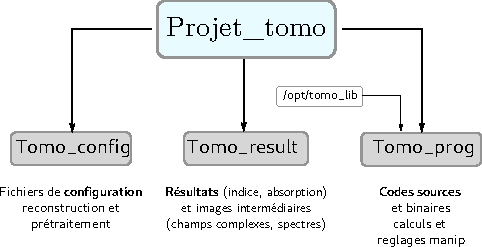
\includegraphics[]{images/projet_tomo.pdf}
 \caption{Chemins utilisés par les programmes de reconstruction}\label{chemin_utile}
\end{figure}

\section{Les programmes utiles}
\subsection{Noms et fonctions}
L'acquisition des hologrammes, la reconstruction et le traitemede ces hologrammes reposent sur différents programmes appelés par l'interface graphique. Tous les binaires ont un nom commençant par \code{tomo\_}
\begin{table}
\begin{center}

{\small{
\begin{tabular}{|l|l|}	\hline
	Nom & Fonction \\\hline
\code{tomo\_gui}	& Interface graphique  \\\hline
\code{tomo\_manip}	& Acquisition \\\hline
\code{tomo\_pretraitement}	& Calcul phase/amplitude\\	\hline
\code{tomo\_reconstruction}	& Calcul de l'image 3D \\	\hline
\code{tomo\_GPS}	& Algo itératif sous contraintes \\ \hline
\code{tomo\_show\_fourier}	& Image caméra et spectre \\	\hline
\code{tomo\_set\_flower}	& Tension miroir \\	\hline
\end{tabular} 
}
}

\end{center}
\caption{Programmes utilisés pour réglages et acquisition}
\end{table}
	
L’ensemble des chemins utiles au fonctionnement est lu dans 
\code{\$HOME/.config/gui tomo.conf}, normalement configuré une seule fois à l'installation du PC.

Les paramètres sont réglables dans l'interface graphique ou directement dans les fichiers de config : \code{recon.txt}, \code{config\_manip.txt}

Les bibliothèques complémentaire (labjack, caméra) sont  dans 
\code{/opt/tomo\_lib} et \code{/opt/pleora}.





Une acquisition + reconstruction peut être faite en console en lançant :
\begin{enumerate}
	\item \code{tomo\_manip}
	\item  \code{tomo\_pretraitement}
	\item  \code{tomo\_reconstruction}
\end{enumerate}
ou en cliquant sur les boutons correspondant dans l'interface graphique.
\subsection{Dépendances}

Diverses bibliothèques doivent être installées :

\begin{itemize}
	\item pleora/GENicam pour la caméra
	\item fftw3 pour la FFT.
	\item libtiff
	\item openCV
	\item exodriver labjack 
	\item wxWidgets pour l'interface graphique
\end{itemize}
 La variable d’environnement \code{\$LD\ LIBRARY\ PATH } ou les fichiers de réglages de chemins  (/etc/ld.conf, .profile) doit être réglés en conséquence.

Les dossiers utilisés par ces programmes sont indiqués sur la figure \ref{chemin_utile}.
\section{Réglages optiques}

L'illumination de Kohler doit être vérifiée (Fig.\ref{kohler}). Elle assure la conjugaison entre le plan objet, le capteur caméra, les diaphragmes de champ.


\begin{figure}
	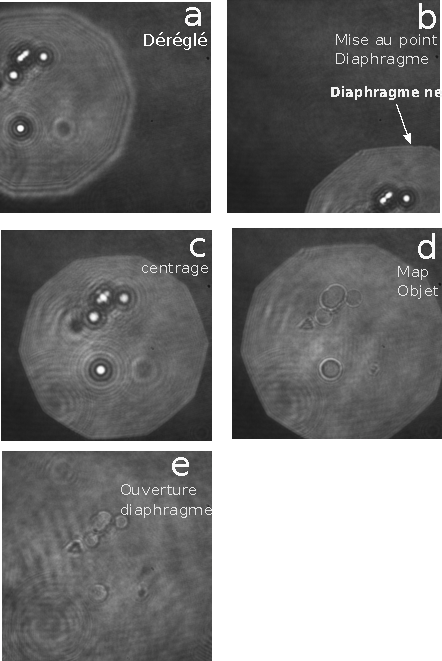
\includegraphics[]{images/Kohler/kohler.pdf}
	\caption{Réglage de l'illumination}\label{kohler}
\end{figure}

Étapes à suivre :
\begin{enumerate}
	\item Kohler déréglé
	\item Mise au point du diaphragme de champ à l'aide du $z$ objectif.
	\item centrage à l'aide des déplacement s$x$, $y$ de l'objectif.
	\item Mise au point objet à l'aide du $z$ platine objet.
	\item Ouverture du diaphragme de champ
\end{enumerate}
	
\section{Correction des aberrations}

Lors du prétraitement, les aberrations résiduelles
sur l’illumination peuvent être corrigées en analysant le fond des acquisitions, dont la phase est supposée plane. L’écart à la planéité fournit le polynôme de correction des aberrations. 

\begin{figure}
	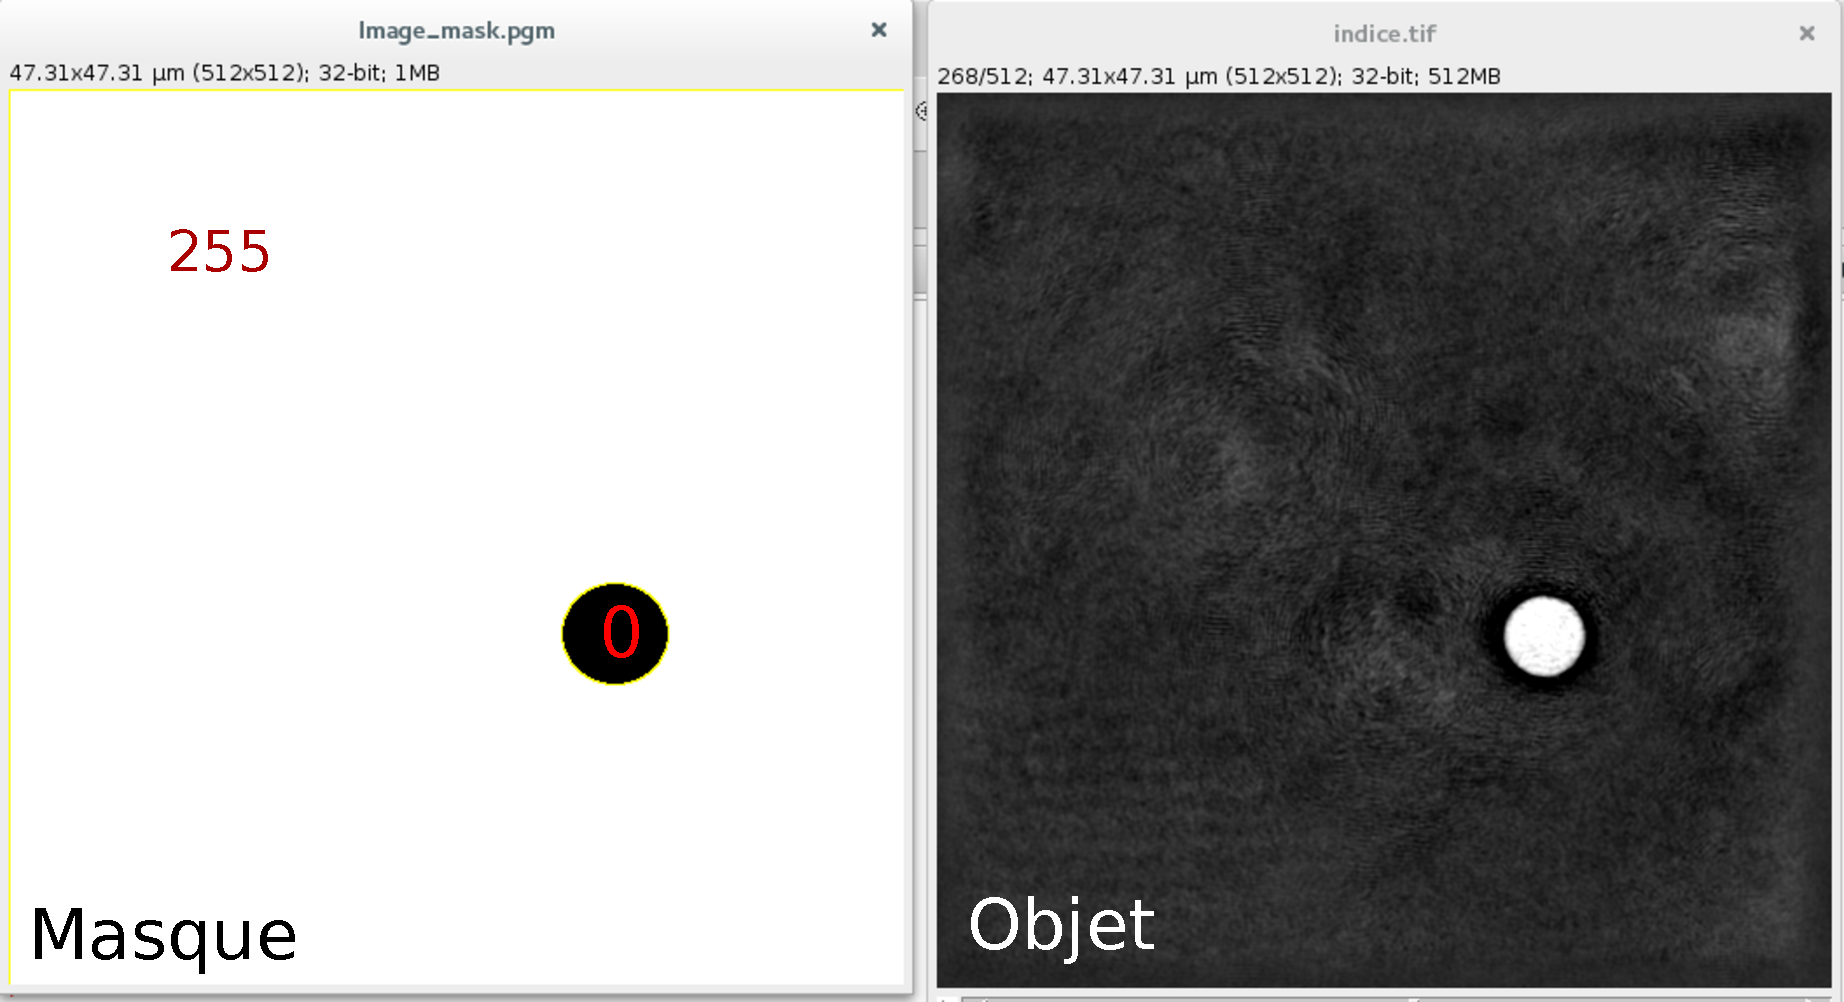
\includegraphics[scale=0.28]{images/masque_aberration.pdf}
	\caption{Masque binaire pour la correction d'aberration}\label{aberration_masque}
\end{figure}

Pour fonctionner de façon optimale, la correction d’aberration nécessite un masque 8 bits (fig.
\ref{aberration_masque}) séparant l’objet (valeur=0) du fond (valeur=255), fourni par l’utilisateur. Il doit être placé dans le dossier d’acquisition  et appelé \code{Image\_mask.pgm}.
En l’absence de masque fourni par utilisateur, un masque unité est généré : il inclut l’objet, la correction n’est donc pas optimale. Le masque peut-être
créé sous \code{ImageJ} grâce aux champs complexes fournis par \code{tomo\_pretraitement}.

\section{Interface graphique}

\begin{figure}
	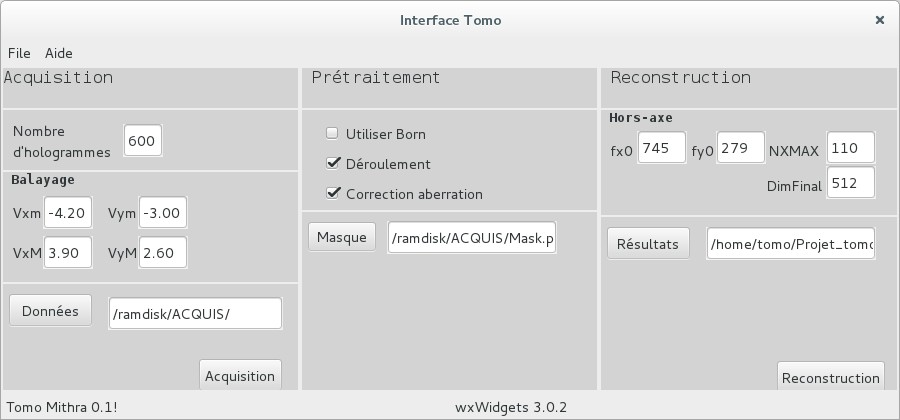
\includegraphics[scale=0.28]{images/Interface_Tomo.jpg}
	\caption{Interface graphique}\label{tomo_gui}
\end{figure}

Elle permet de faire une acquisition et de régler différents paramètres (Fig. \ref{tomo_gui}).
Quelques mots-clés : 

\begin{itemize}
	\item Rytov. L’approximation de Rytov est
	meilleure pour les objets épais ($>$5μm), mais
	nécessite un déroulement de phase. Défaut=1.
	\item C\_ABER. Corriger les aberrations. Défaut=1.
	\item Volkov. Le déroulement de phase peut être réalisé par
	la méthode Volkov (méthode globale, utilisant l’es-
	pace de Fourier) ou Herraez (méthode dans l’espace
	direct, utilisant le chemin de ”meilleure confiance”.  Défaut=1.
	\end{itemize}

Les tensions de balayage et réglages Hors axe ne devrait pas être modifiées après installation de la machine. 
Les fenêtres des différents programmes sont fermables par ALT+F4.
\section{Réglages caméra Gigabit}

La caméra est sur la 2è carte ethernet (pci). Les jumbo frames (trames géantes) doivent
être activées avec l’option MTU=9000, sinon la caméra
plafonne à 80 IPS au lieu de 90. La carte ethernet
prends une adresse locale de type 169.168.0.2. Il
faut enfin fixer une adresse IP pour la caméra, sur le même sous réseau.

\section{Schéma de principe}
\begin{figure}[ht]
	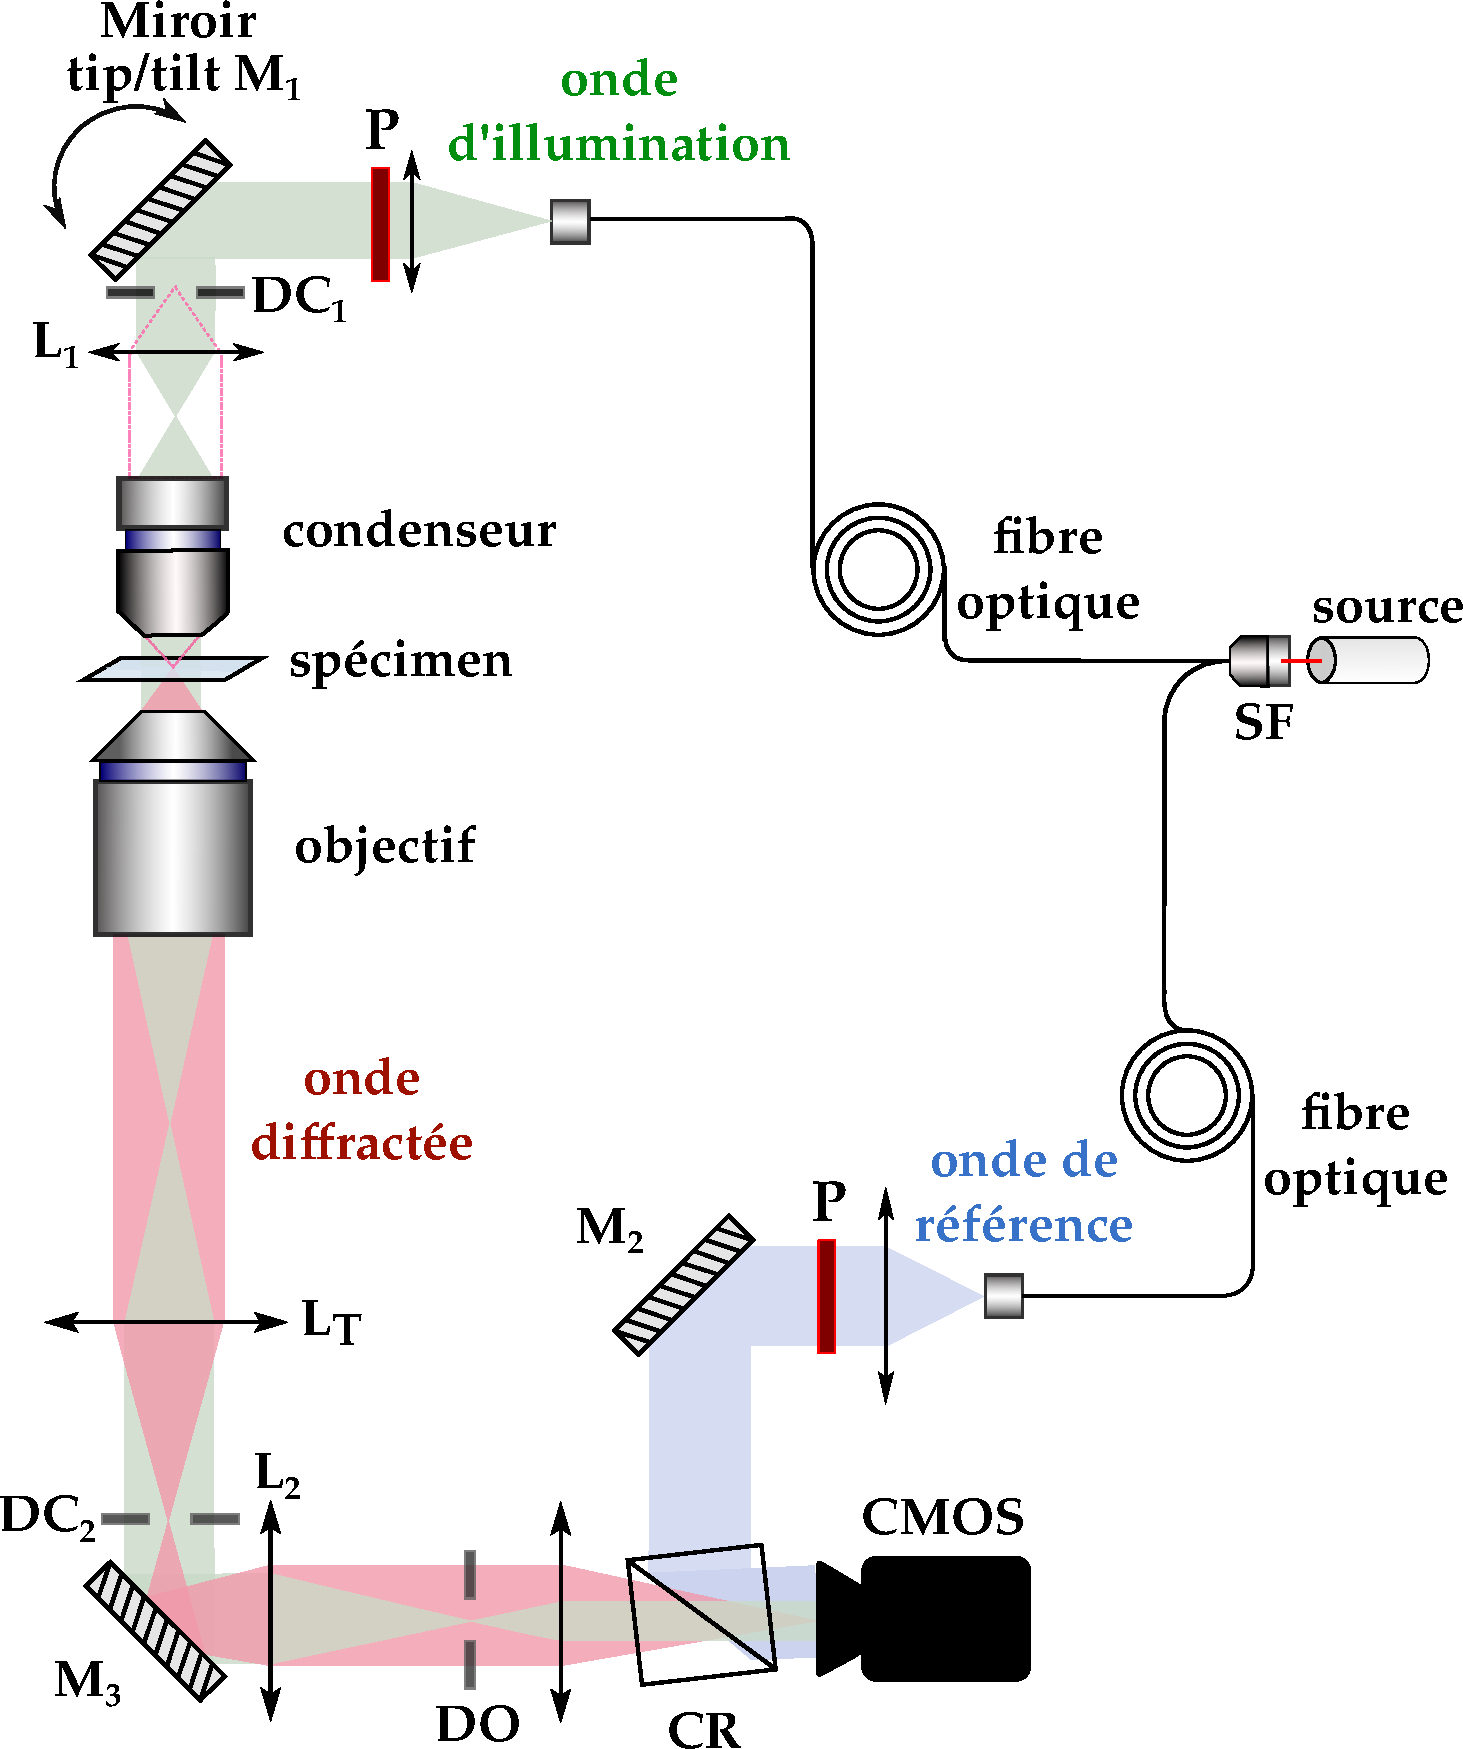
\includegraphics[scale=0.36]{images/schema_manip2.pdf}
	\caption{Microscope tomographique en transmission}\label{schema_manip}
\end{figure}
Le montage repose sur un interféromètre de Mach-Zehnder fibré. Un séparateur fibré \code{SF} crée une onde d'illumination plane et une onde de référence. Le miroir de balayage \code{M$_1$} permet de parcourir la pupille arrière du condenseur avec un point focal (la lentille de tube \code{L$_{T1}$} focalisant l'onde), créant une série d'illuminations planes sur le spécimen. L'objectif collecteur et sa lentille de tube reforment l'image au niveau du diaphragme de champ \code{DC$_2$}. Un doublet de lentille afocal permet de contrôler le grandissement final et donc l'échantillonnage. Le diaphragme d'ouverture \code{DO} permet un filtrage complémentaire.   
Enfin, l'onde de référence et objet sont recombinées par le cube recombinateur \code{CR}, et l'image formée sur la caméra.

\end{document}
